\newpage
\section{Экспериментальная часть}
\subsection{Макет шагового привода}

Макет состоит из спроектированного механического стенда
(см. \ref{sec_stand_construction}) и макетной платы
Texsas~Instruments~C2000~Piccolo~F28035.
В качестве шагового двигателя используется двигатель, запланированный для работы
в реальном приводе~--- Telco~Motion~4T5618M308 (табл. \ref{engine_params}), в
качестве датчика~--- импульсный датчик ЛИР--137А 6250--05--ПИ
(табл. \ref{encoder_params}).

Схема экспериментального стенда изображена на рис.
\ref{pic_experim_stand_scheme}, где

\begin{enumerate}
        \item Датчик углового положения
        \item Источник питания
        \item Муфта соединительная
        \item Муфта соединительная малая
        \item Объект регулирования
        \item Осцилограф
        \item Персональная ЭВМ
        \item Плата управления
        \item Шаговой двигатель
\end{enumerate}

\begin{figure}[hb]
    \centering
    \centering
    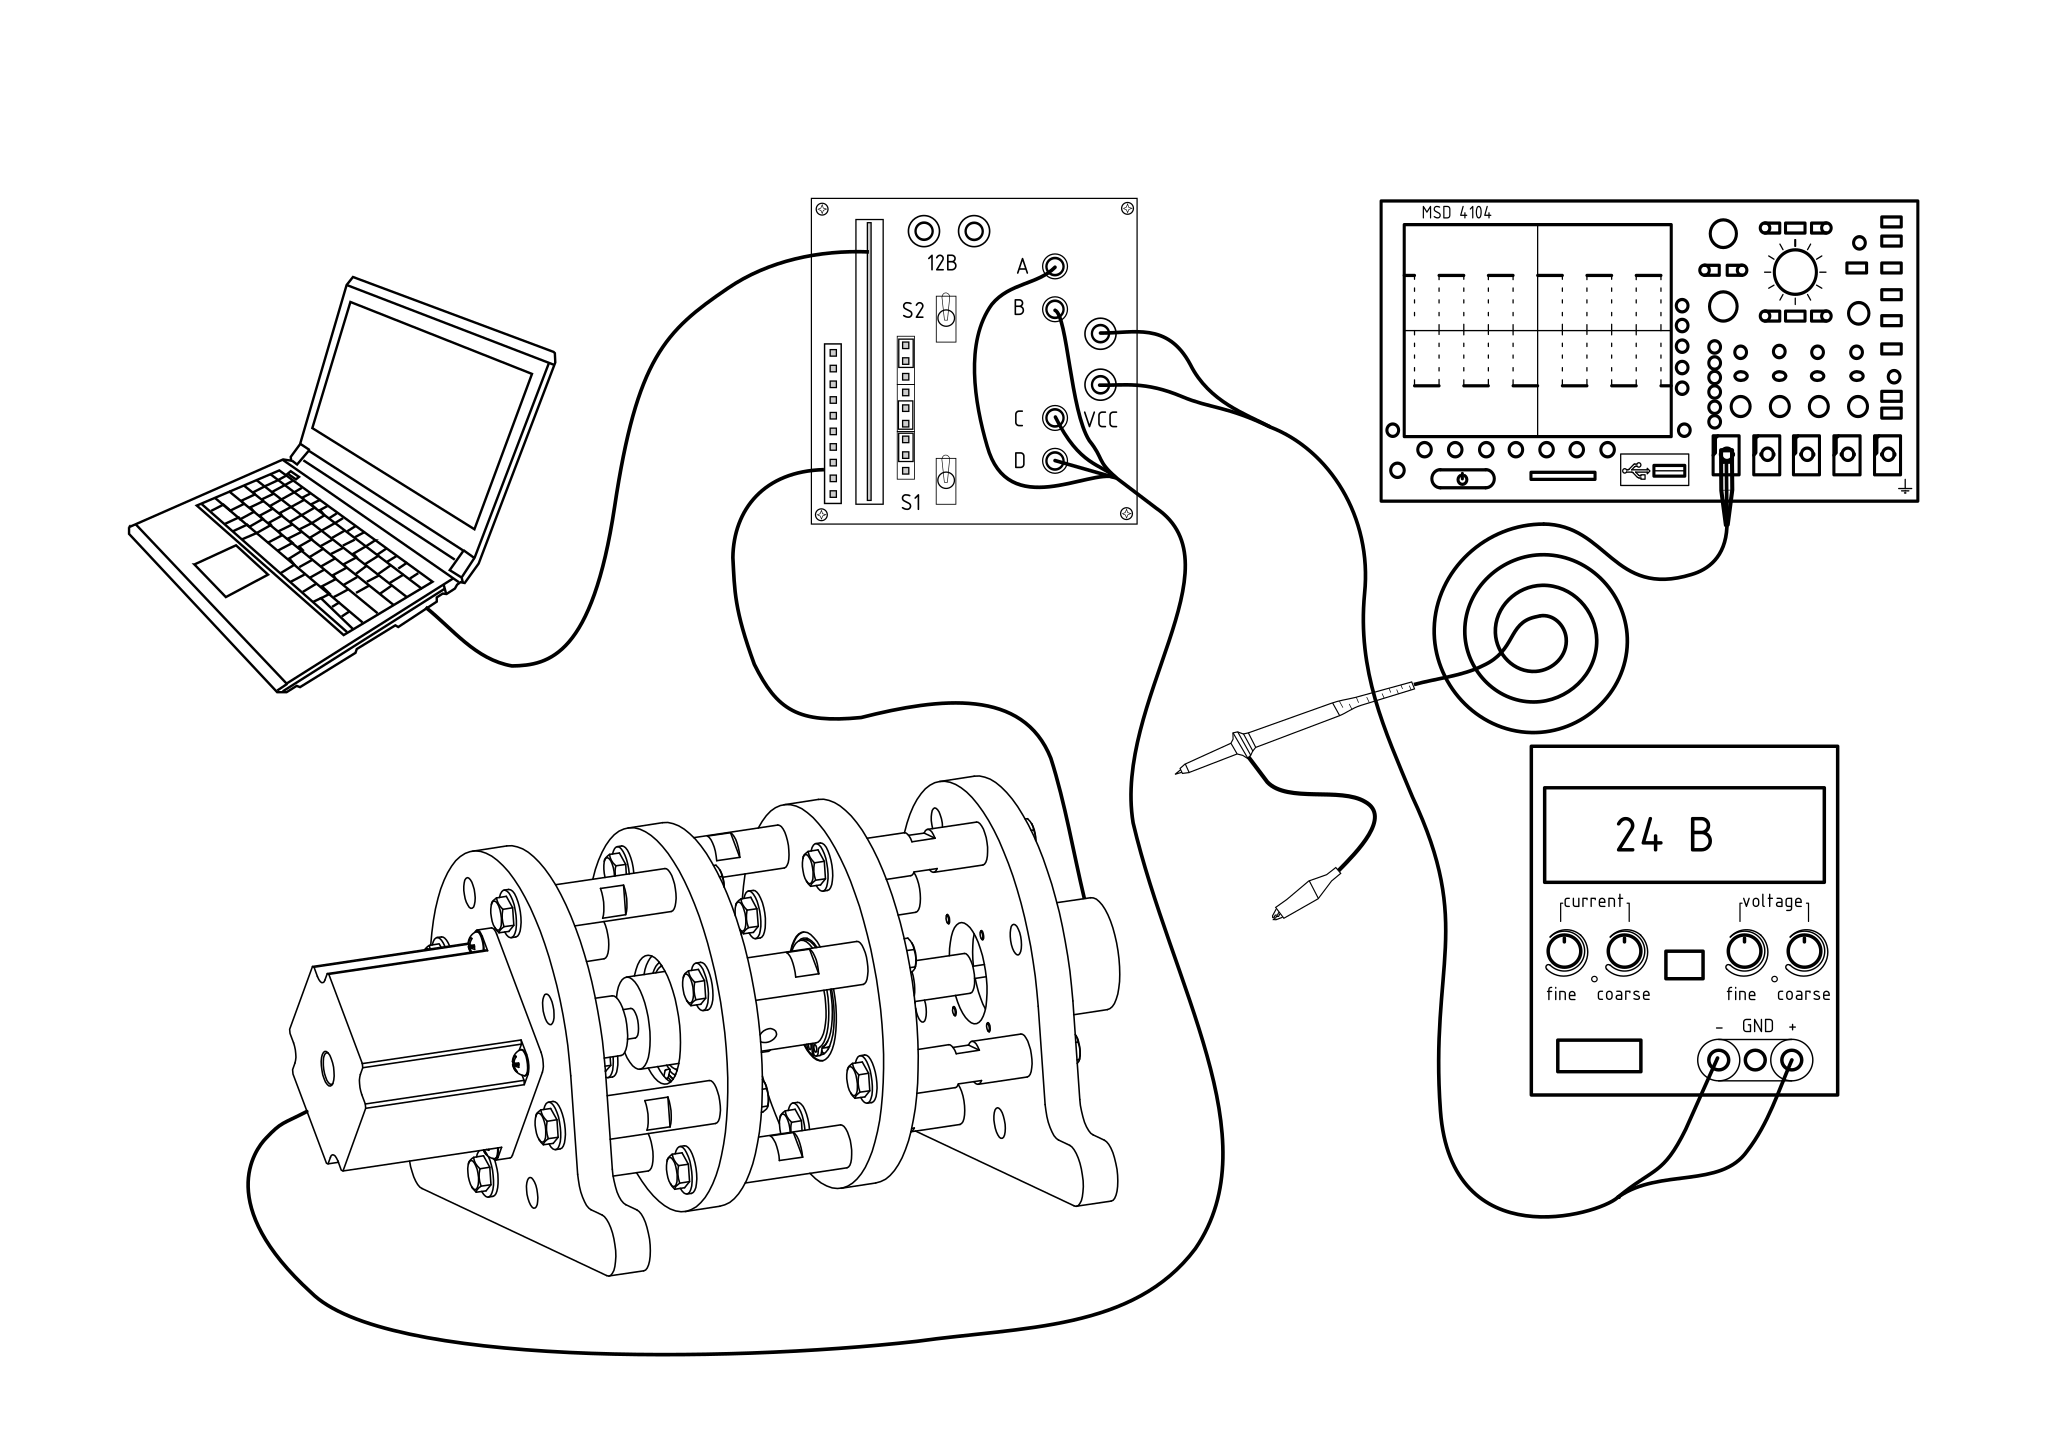
\includegraphics[width=\linewidth, keepaspectratio,
                    clip=true, trim=51mm 21mm 51mm 20mm]
                    {src/pictures/experimental_stand_draft}
    \caption{Схема экспериментального стенда}
    \label{pic_experim_stand_scheme}
\end{figure}
\subsubsection{Описание экспериментов}

Эксперименты, проводимые на экспериментальном стенде, направлены на оценку
качества управления созданными алгоритмами, получение информации о процессах,
протекающих в шаговом двигателе, а так же верификацию построенных в
\ref{sec_math_modeling} математических моделей.

Большая часть условий проведения экспериментов является общей для всех экспериментов
и описана в табл. \ref{experiments_conditions}.

\begin{table}[ht]
    \centering
    \begin{tabu}{X[l]|X[-1,r]} \hline
        Алгоритм переключения шагов                             & Одношаговый   \\
        Алгоритмический шаг двигателя, град.                    & 1.8           \\
        Момент инерции нагрузки, приведённый к ротору двигателя,
        $\text{кг} \cdot \text{мм}^2$                           & 55            \\
        Напряжение питания двигателя, В                         & 24            \\
        Частота ШИМ, кГц                                        & 58.5          \\
        Число отсчётов датчика углового положения на оборот     & 25000         \\
        Целевое положение, отcчёты энкодера                     & 101250        \\
        Число точек снимаемых характеристик                     & 1000          \\
        Контур по току                                          & Отключён      \\
        Контур по скорости                                      & Отключён      \\
        Алгоритмы плавного разгона и торможения                 & Отключены     \\ \hline
    \end{tabu}
    \caption{Общие условия проведения экспериментов}
    \label{experiments_conditions}
\end{table}

Каждый эксперимент включает в себя наблюдение за процессами, протекающими
при <<старте>> привода и при достижении целевой точки (<<финиша>>).

Все проведённые эксперименты можно разделить на две части - эксперименты с
использованем алгоритма управления с ОС по положению и эксперименты
с использованием бездатчикового управления.

Эксперименты с использованием ОС по положению проводены для трёх значений
углов коммутации $\theta_\text{ком} = 1, ~1.3, ~1.5$ и для двух значений
коэффициентов заполнения ШИМ: $\zeta = 0.033, ~0.1$

Эксперименты с использованем бездатчикового управления проведены при периоде
переключения шагов 20 мсек, для двух значений коэффициентов заполнения ШИМ:
$\zeta = 0.033, ~0.05$

\subsubsection{Результаты экспериментов}

Успешно получен ряд экспериментальных данных во всех намеченных сценариях.
Система работает стабильно, без выпадений из синхронизма.
Из особенностей стоит отметить большую зашумлённость сигнала по скорости,
возникающую из-за того что величина скорости получена дифференцированием сигнала
по положению.

\subsubsection{Выводы по экспериментальной части}

Анализ результатов экспериментов показал преимущества управления с ОС
по положению с использованием различных углов коммутации. Использование ОС
по положению позволяет в значительной степени улучшить профиль скорости
и сделать движение более равномерным.

Оба используемых алгоритма можно считать способными к управлению приводом, но
для управления на высоких скоростях необходимо введение ОС по скорости, а так же
алгоритмов плавного разгона и торможения. Это так позволит значительно повысить
точность позиционирования при средних и малых скоростях.

Для более подробного анализа необходимо получить данные по протекающим в фазах
шагового двигателя токах.

В целом полученные результаты совпадают с результатами, полученными на основе
математических моделей привода (см. \ref{sec_math_modeling}), тоесть можно говорить
об успешной верификации моделей.
